% !TeX spellcheck = en_US
\documentclass[12pt,a4paper,twocolumn]{article}
\usepackage[utf8]{inputenc}
\usepackage[T1]{fontenc}
\usepackage{amsmath}
\usepackage{amssymb}
\usepackage{graphicx}
\usepackage{fancyhdr}
\usepackage[english]{babel}
\usepackage{geometry}
\usepackage[dvipsnames]{xcolor}
\usepackage[english]{babel}
\usepackage{hyperref}
\usepackage{float}
\usepackage{csquotes}
\usepackage[style=numeric, url=true, doi=true, isbn=false, backend=biber, sorting=none]{biblatex}
\usepackage{array}

\newcolumntype{L}{>{\centering\arraybackslash}m{5.5cm}}

\title{Training of a Convolutional Variational Autoencoder for PPG signals}
\author{Lorenzo Barsotti}

\addbibresource{bibliografia.bib}
%\bibliographystyle{plain}
\geometry{ margin=2cm}
\pagestyle{fancy}
\begin{document} \thispagestyle{empty}
	%\maketitle
	
	\twocolumn[{%
		\begin{@twocolumnfalse}
		\huge \bfseries Training of a $\beta - $Convolutional Variational Autoencoder for PPG signals 
		\begin{flushright}
			\large \bfseries Author: Lorenzo Barsotti	
		\end{flushright}
		
			\begin{abstract}
				
				Photoplethysmography acquired through the camera and the diode of a smartphone is a cheap and non invasive method that can be used to estimate the vascular aging of a patient. In this study we would like to apply a $\beta-$Convolutional Variational Autoencoder to perform this task. In this report are shown the best parameters and the best structure of the Neural Network with the best reconstruction performances of the peak. The final results show that it is possible to separate partially in the latent space the PPG of the young people from one of the older ones. In particular, it is possible to recognize the main feature that allows us to distinguish a PPG belonging to a young person, in the presence of an accentuated concavity in the peak, identified with the \emph{dicrotic notch}. The results coming from the application of Deep Learning to PPG could lead to the diffusion of PPG as a screening tool.
				
			\end{abstract}
		\end{@twocolumnfalse}
	}]

	\section{Introduction}
		The purpose of this project is to estimate the biological age of a patient, from its photoplethysmogram. A photoplethysmogram is the optically obtained signal related to the changes of volume in the blood vessels (Section \ref{ppg_intro}). In order to perform the age estimation we used a database composed of 4769	photoplethysmograms of as many patients, and a \emph{ $\beta-$Convolutional Variational Autoencoder}. This is a particular case of \emph{Deep Neural Network} (DNN) as it will be described in the Section \ref{vae:intro}. To develop, train and validate the Convolutional Neural Network it was used a MacBook Air M1 2020 in the configuration with 7 core GPU and 8 GB of memory \cite{MBA} and Python 3.9.13: miniforge3 \cite{miniforge-doc} and Tensorflow 2.9.0 \cite{tensorflow2015-whitepaper}.
	\subsection{Photoplethysmography}
		\label{ppg_intro}
		\emph{Photoplethysmography} is a technique that use light in order to detect changes in volumes in blood vascular vessels. A \emph{Light Emitting Diode} (LED) illuminates a high vascularized body part covered by a thin layer of skin, usually a fingertip, and a photodiode measures the amount of light transmitted or reflected. In the particular case of this project, the data were taken with the camera module of a smartphone: the LED illuminates a fingertip and the camera records the backscattered light \cite{Matsumura2015}.
		 
		A \emph{photoplethysmogram} (PPG) is the plot of the recorded data of the photodiode. It is a graph in which we are able to see how  the blood vessels' volume changes over time. After some data manipulations, such as denoising, and application of a \emph{high-pass} filter, the corresponding graph looks like the one in Figure \ref{fig:ppgexample}.
		\begin{figure}[h!]
			\centering
			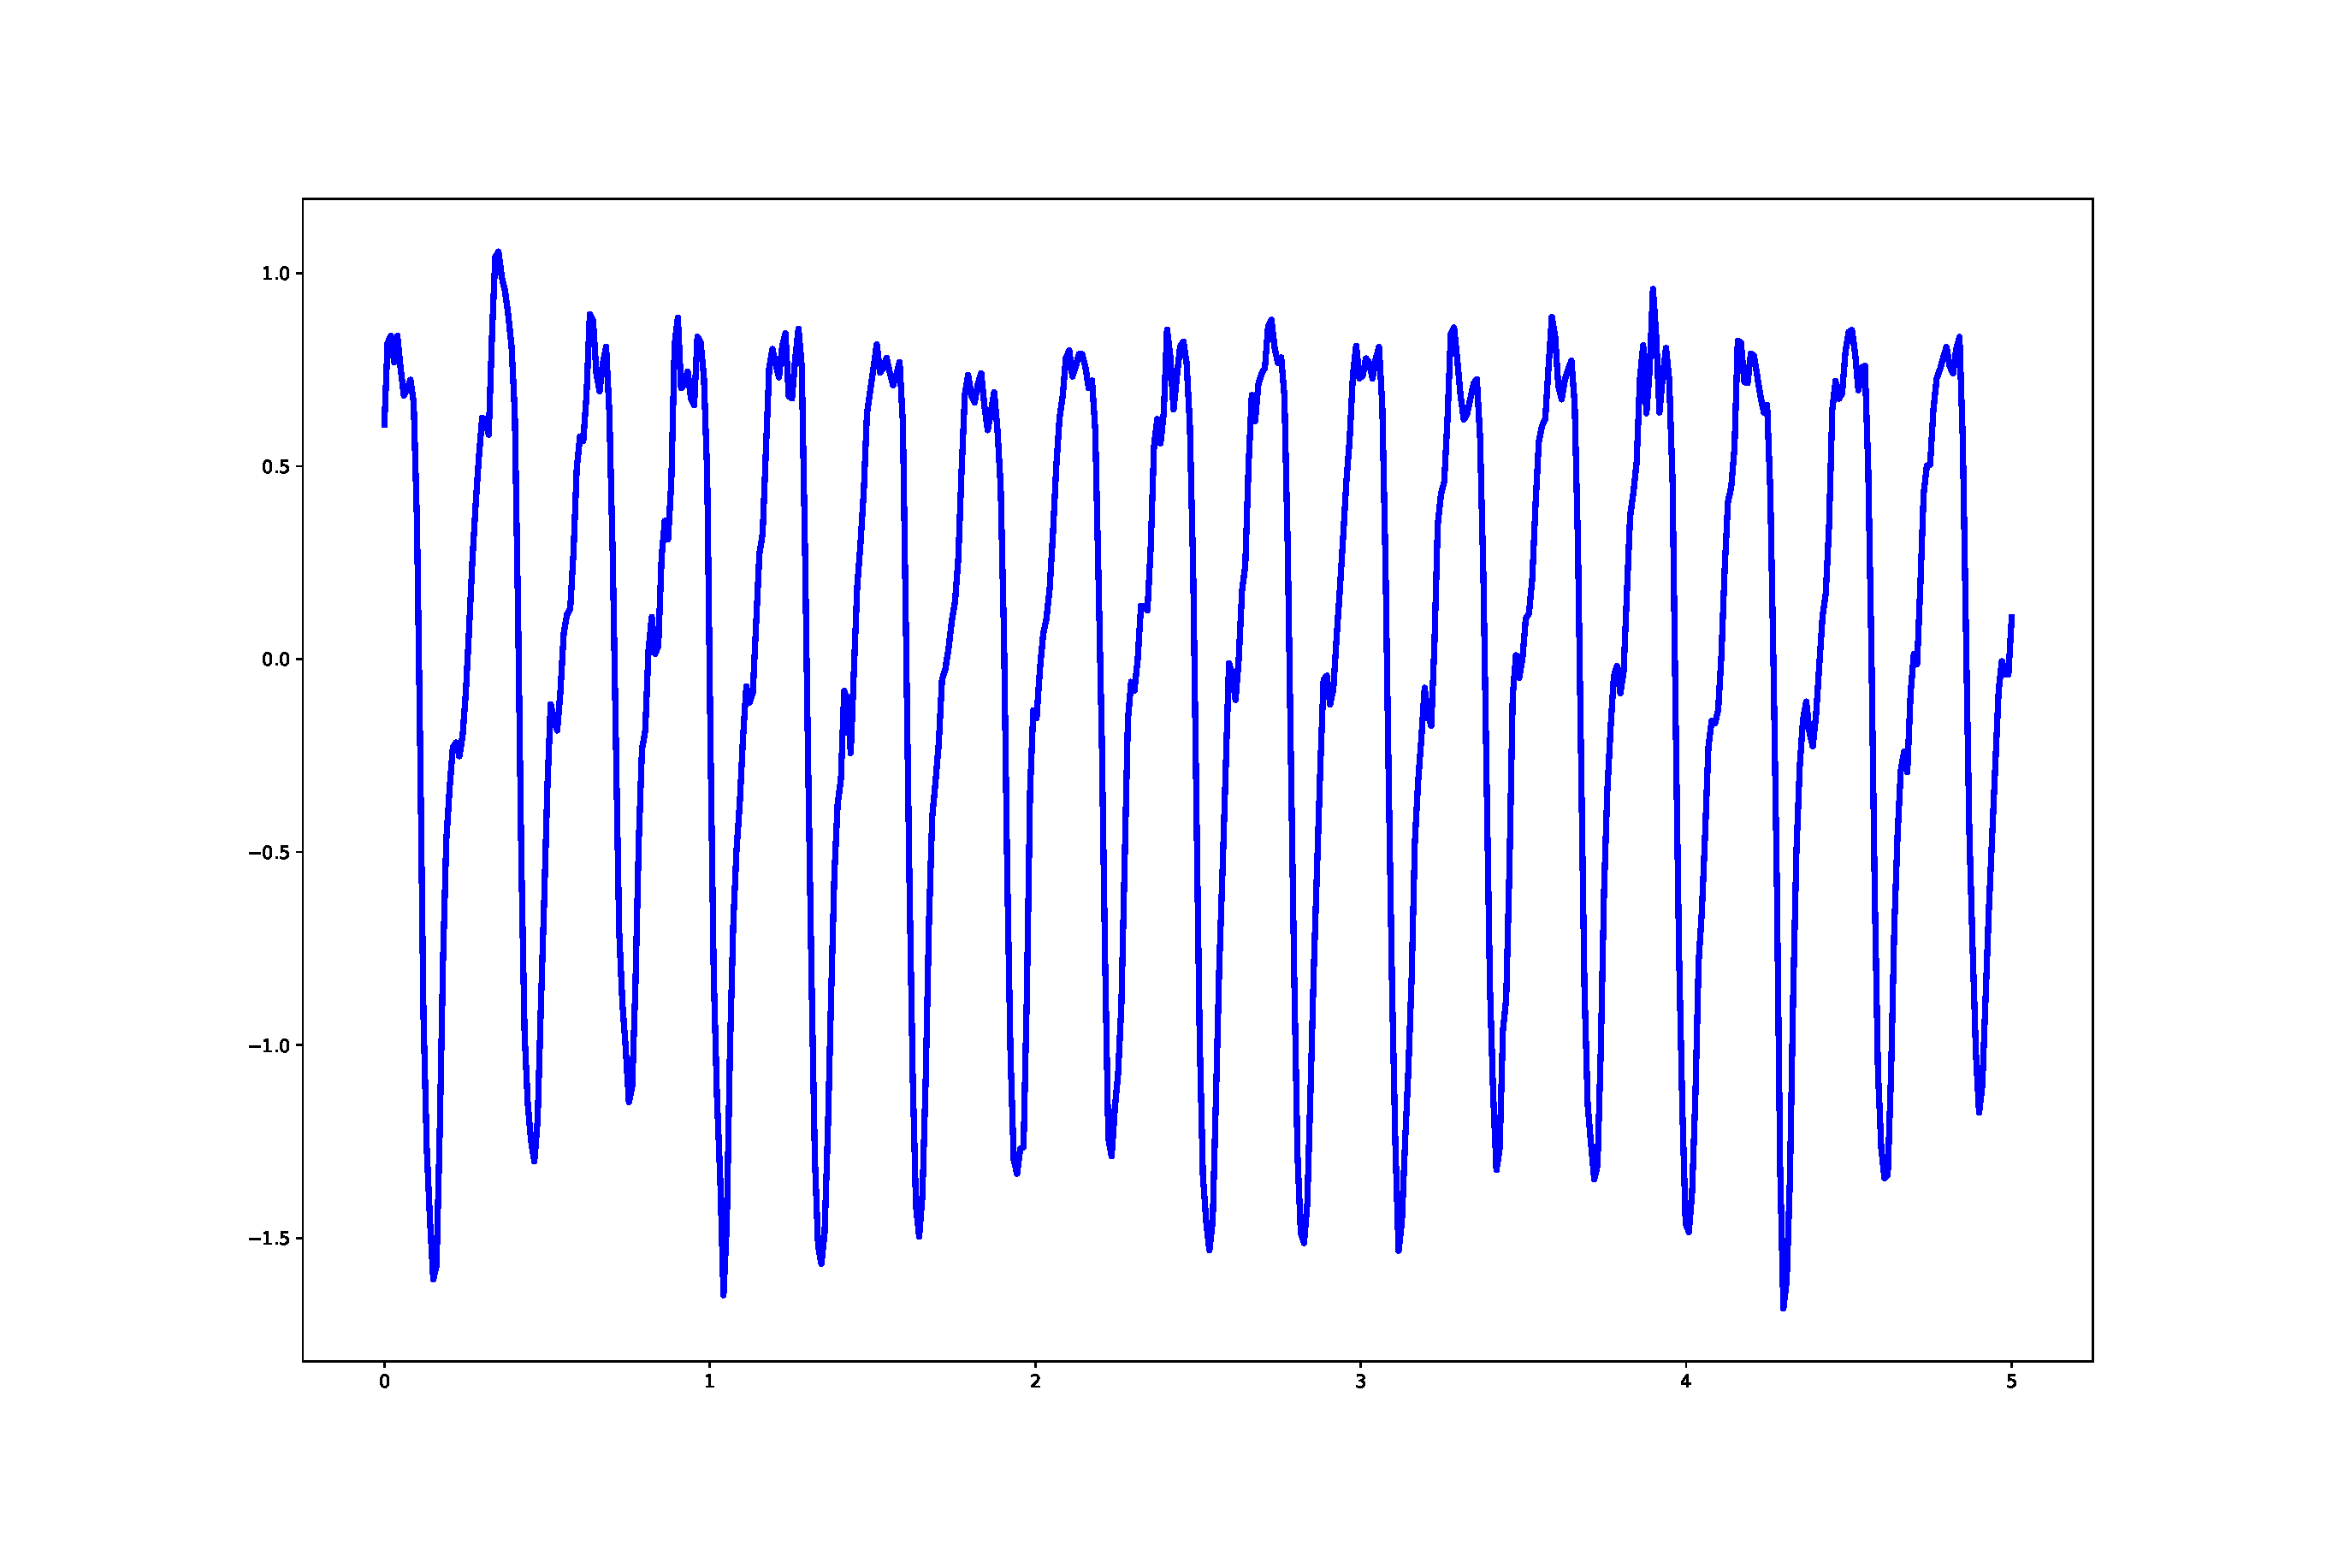
\includegraphics[width=1\linewidth]{images/ppg_example2}
			\caption{Example of a photoplethysmogram present in the database. The figure shows only the first part of the plot, that is much larger.}
			\label{fig:ppgexample}
		\end{figure}
		\subsection{$\beta-$Variational Autoencoder}
		\label{vae:intro}
		The	\emph{Variational Autoencorder} (VAE)  \cite{vae_paper} is an architecture of \emph{Deep Neural Network}. It can be used with different purposes, but in this project it has been used to perform an  \emph{unsupervised learning}. This means that, during the training, we don't provide as input the ages corresponding to the PPGs.
		
		In this study, it has been used a \emph{Convolutional Vaeriational Autoencoder} (CVAE), that is a particular case of VAE, in which are performed convolutional operations.  A CVAE can be represented by the scheme in Figure \ref{fig:vaebasic} \cite{vae_scheme}, where we can see that it is composed by several \emph{layers}, classified in three categories:
		\begin{itemize}
			\item \textbf{encoder}, the data are provided to the \emph{input layer} in the form of a tensor, with a shape equal to (number of inputs, input height, input width, number of channels). This initial layer transmits the data to the \emph{encoder}, that perform convolutions operations (Section \ref{convolution}), in order to compress the initial data. It is crucial to understand that the \emph{encoder} maps the initial data to a multivariate Gaussian distribution. This means that, at the end of the \emph{encoder} network, the output is composed by two vectors: mean, and variance, of a certain dimension.
			\item \textbf{latent space}, the compressed data, under the form of distribution, lie in the \emph{compressed space}, also called \emph{latent space}. The compression phase can be lossy or not, depending on the structure of the \emph{encoder}. If the compression is lossy, it means that not all the information of the input data is maintained so, starting from the compressed data, it is not possible to perfectly reconstruct the initial ones.
			\item \textbf{decoder}, it has the opposite task of the \emph{encoder}, performing \emph{deconvolution} operations to the input. With these operations, the \emph{decoder}, has to decompress the \emph{latent space} in order to reconstruct an output as similar as the input. In this phase, a value is sampled randomly from the normal distribution of the latent space and, with this values, an output is reconstructed.
		\end{itemize}
	
		\begin{figure}[h!] 
			\centering
			\includegraphics[width=0.9\linewidth]{images/Basic-structure-of-Variational-Autoencoder-VAE_W640}
			\caption{Structure of a VAE. It is possible to distinguish the \emph{encoder} that, in the particular case of a \emph{Convolutional}$-$ VAE, performs convolution operations, the \emph{ latent space}, in which the important information are contained, and the \emph{decoder}, that tries to reconstruct the output starting from the latent space and provide us the Neural Network output.}
			\label{fig:vaebasic}
		\end{figure}
	
		\subsubsection{Convolutions}
		\label{convolution}
		To see how a convolutional layer operates, let's consider the case in which the input data is made of images, that is the case of two dimensional arrays, and then the extension to the case of one dimensional arrays will be trivial. 
		\begin{figure*}[ht]
			\centering
			\includegraphics[width=0.7\linewidth]{images/A-typical-2D-convolution-operation_W640}
			\caption{Example of how a \emph{kernel} (or \emph{filter}) matrix  convolution works. The source matrix is convoluted with the \emph{kernel} matrix. This leads to a number that becomes the output value of a pixel.}
			\label{fig:kernel}
		\end{figure*}
	
		A convolution consists in convoluting a \emph{source matrix} $S$, sub-matrix of the input image, with a predefined \emph{kernel matrix} $K$, square matrix of the same dimensions of $S$ (Figure \ref{fig:kernel}, \cite{kernel_cov}). The two matrices usually are square matrices with an odd number (\emph{kernel dimension}) of rows and columns. The convolution of $S$ with $K$ is defined as \cite{8308186}:
		$$C := \sum_{i=0}^{N_{col}}\sum_{j=0}^{N_{row}} S_{ij}K_{ij}$$
		
		This number is the value of a pixel of the new convoluted matrix. If this process is repeated moving the sub-matrix along the image, we obtain a convoluted matrix. An analogue process, but finalized to increase the dimension of the input, is performed in the \emph{decoder}.
		
		Some parameters, such as the \emph{padding} and the \emph{stride}, determine how the convolution is performed:
		\begin{itemize}
			\item \emph{padding}, this parameter sets the boundary conditions. It fixes the way we have to perform the convolution for the pixels at the boundaries of the image. A padding \emph{valid} means  that the convolution operations are performed only on the real pixels of the image, as it can be seen in Figure \ref{fig:kernel}, while a padding \emph{same}, is achieved by adding a column on the left side, a column on the right side, a row at the top and a row at the bottom of the image, containing all zeros.
			\item \emph{stride}, this parameter is used to set the step to be performed during the convolution af the whole image. If $stride=2$, it means that a convolution  is performed every two pixels. In other words, it says how many pixels we have to move the source matrix along the image to perform the convolution.
		\end{itemize}
		
		As said before, the extension to the one dimensional case is trivial. In that case, the kernel matrix becomes an array of values.

		\subsubsection{Reparametrization Trick}
		The \emph{decoder} samples randomly from the distribution in the \emph{latent space}, getting a variable $z$. Since it is impossible to \emph{back-propagate} through a stochastic node and learn the parameters of the distribution, the  \emph{reparametrization trick} is used  (Figure \ref{fig:rep_trick}, \cite{rep_trick}). The sampling of the variable $z$  follows the expression:
		 $$z = z_{mean} + \sigma\times\varepsilon$$ 
		 where $\varepsilon$ is a normally distributed variable, $z_{mean}$ and $\sigma$ are the parameters of the distribution in the latent space. Performing this operation allows to move the stochasticity from the node we have to backpropagate through, to the variable $\varepsilon$.
		 %where the stochasticity is moved from the node through we have to backpropagate, to the variable $\varepsilon$, that is a normal distributed variable. 
		 In this way, the stochasticity is preserved, but it is now possible to backpropagate and learn the parameters of the distribution.
		 
		\begin{figure*}[t]
			\centering
			\includegraphics[width=0.7\linewidth]{images/VAE-reparameterization-trick_W640}
			\caption{In this Figure it is possible to appreciate the differences in the two approaches for the sampling of the latent distributions. On the left side we have the original approach, where the stochasticity is present in the $Z$ node. This prevent the backpropagation and the learning of the NN. On the left side, the stochastic part is moved through the parameter $\varepsilon$, allowing the backpropagation through the node $Z$.}
			\label{fig:rep_trick}
		\end{figure*}
	
		\subsubsection{Loss Function}
			In the training of a $\beta-$VAE, we try to learn the parameter of a distribution. In order to do that, we use a loss function composed by two terms \cite{9244048}:
			\begin{itemize}
				\item \emph{Reconstruction}: that ensures the similarity between the input and the output.
				\item \emph{Regularization}: that helps to create a well-structured latent space, having a beneficial effect in the disentanglement of the latent representation \cite{9244048}.
			\end{itemize}
			For the \emph{reconstruction loss}, the \emph{Mean Square Error} (MSE) was used.
			In the VAE, the \emph{regularization term} is given by the \emph{Kullback-Liebler} \emph{Divergence} (KL), that measures the distance between two distributions \cite{KL}. In particular, it quantifies the loss of information that would occur by using the Gaussian as an approximation of the distribution obtained from the data.
			
			The structure of this NN is called $\beta-$VAE because the regularization term is multiplied by a parameter $\beta$. By modifying the value of $\beta$, we focus on the reconstruction or on the regularization term.

		\section{Methods}
		\subsection{The database}
			The database \cite{database} contains data coming from 4769 patients. In the database, there are 107 features, the most important of these (even if not all of them have been used) are: age, sex, \emph{Body Mass Index} (BMI), BPM, if the person smoke or not,  weight and a quality score of the PPG (the lower, the better). The data were taken through an app and the acquisition was voluntary, meaning nobody checked if the acquisition was well performed or not. There are several factors, such as the voluntary and involuntary movements of the patient, that could lead to a worse result. 
			%The quality of the PPG depends from several factors, for example the pressure the person makes on the camera of the smartphone, or the inclination of the finger respect to the camera. For this reason the PPG are classified with a number called quality.  
			The smaller this parameter  is, the better and cleaner the PPG is. A PPG is saved in two arrays of the same length: the first one contains the time at which the signal was sampled, while the second one contains the value of the signal at the moment of the sampling.
			
			Ideally, to train the NN, an homogeneous database should be used, in which the data of the patients are uniformly distributed, with respect to the sex, age, BMI\dots If it is not the case, the NN might have a bias and thus, it might better recognize some kind of PPG. In Figure \ref{fig:agehistogram} it is possible to observe the age distribution of the patients. We can see that there is a lower limit set at the age of 18 and that there are few very old patients.
			In the database are present 2997 male and 1772 female.
			\begin{figure}
				\centering
				\includegraphics[width=0.99\linewidth]{images/Age_Histogram}
				\caption{Distribution of the ages between the patients. In green there are the entries used to train the NN, while in red the entries excluded from this process. }
				\label{fig:agehistogram}
			\end{figure}
				\begin{table*}[h!]
				\centering
				\begin{tabular}{|c|c|L|}
					\hline
					\rule[-1ex]{0pt}{2.5ex} \textbf{Parameters} & \textbf{Best Value} & \textbf{Notes}\\
					\hline
					\rule[-1ex]{0pt}{2.5ex} Number of layers (encoder) & 12 & \\
					%\hline
					\rule[-1ex]{0pt}{2.5ex} Number of layers (decoder) & 14 &\\
					%\hline
					\rule[-1ex]{0pt}{2.5ex} Activation function & ELU  & For the first convolutional layer of the encoder the activation function is RELU\\
					%\hline
					\rule[-1ex]{0pt}{2.5ex} Numbers of filters & 1  & \\
					%\hline
					\rule[-1ex]{0pt}{2.5ex} Padding (encoder)& valid &  \\
					%\hline
					\rule[-1ex]{0pt}{2.5ex} Padding (decoder)& same &  \\
					%\hline
					\rule[-1ex]{0pt}{2.5ex} Kernel initializer & random normal  & seed = 42 \\
					%\hline
					\rule[-1ex]{0pt}{2.5ex} Kernel size & 5 &\\
					%\hline
					\rule[-1ex]{0pt}{2.5ex}  Loss functions & MSE and KL &\\
					\rule[-1ex]{0pt}{2.5ex} $\beta$ &  $0$, $0.2$  & $0$ for the first 50 epochs and $0.2$ for the last 50  \\
					%\hline
					\rule[-1ex]{0pt}{2.5ex} Learning Rate & $3\cdot 10^{-3} $&\\
					%\hline
					\rule[-1ex]{0pt}{2.5ex} Optimizer & Nadam &\\
					\hline
					
				\end{tabular}
				\caption{Here are reported all the best parameters used to train the NN.}
				\label{tab:parameters}
			\end{table*}
			\subsection{Preprocessing}
				The signals present in the database were not the raw data recorded by the smartphones, but they were already preprocessed. In particular ,the raw data were detrended, performing an \emph{high-pass} filter, demodulated and denoised. This aims to obtain a normalized and clean signal.

				In order to give a database in which the peaks of the PPGs are recognizable to the NN, we used the quality index to filter them. So we set the quality threshold to 0.005 and we removed all the patients whose PPG quality index was higher than this threshold. The quality index filter was not able to remove a plate PPG, so it was removed manually. After this operation, the number of usable PPGs was 3255, that means that about 1500 PPG were removed.
				
				Since there are patients with very different ages in the database, there could be PPGs of the intermediate ages, with some properties of young people and some of the elders. For this reason, in order to allow the NN to better distinguish the characteristics of these two types of PPGs, the database was divided into three  groups with the same cardinality, based on the age of the patients: the first one contains only the youngest patients, with an age lower than 38, the second one, the people with an age between 38 and 60, and the last one, the oldest people, with an age grater than 60. Then, only the youngest and the oldest groups have been kept in the database, as it can be seen from the colors in the Figure \ref{fig:agehistogram}. 
				
				At the beginning of this project each signal was divided into chunks containing 15 peaks each, but in that way the NN was not able to correctly reconstruct the signal from the latent space. For this reason, the number of peaks in a chunk was reduced to one. At the end, 175816 chunks (and peaks) were available to train, test and validate the network. Each peak was given to the NN, under the form of an array of 64 values, corresponding to the values of the peak in 64 equally divided intervals.
				
				Then, these chunks were randomly splitted into three groups: train, test and validation, whose dimensions were respectively 80\%, 10\% and 10\% of the total chunks.
		
			\subsection{The Network}
			In order to obtain the results that will be shown in Section \ref{Results}, many attempts have been made to tune one parameter at the time and find its best value. The best parameter is the one that maximizes the distance between the clusters in the latent space using as reference the validation dataset, and the ability to reconstruct the peaks. In particular, different tries have been made on the numbers of layers (to see what would happen with a deeper network), on the number of filters, on the activation functions, on the \emph{kernel initiaizer}\footnote{Parameter that determines the initial weights of the NN.}, on the loss function and on the \emph{kernel size}. For the final training of the NN, the structure used was the following: the \emph{encoder} was composed by 12 \emph{convolutional layers}, while the \emph{decoder} had 1 \emph{dense layer} and 13 layers that performed deconvolutions\footnote{A transpose convolutional layer, with a small input tries to reconstruct an output with higher dimension.}. In addition, it is important to underline that the arrays were provided to the Network divided in batches, whose dimension was 128. During the training, the \emph{learning rate} was $3\cdot 10^{-4}$ and it was divided into two phases of $50$ epochs each: the first one had $\beta=0$, while the second one had $\beta=0.2$.
			The other best parameters found for this structure, are resumed in the Table \ref{tab:parameters}. 
			\begin{figure*}
				\centering
				\includegraphics[width=1\linewidth]{images/test_young_old}
				\caption{Here it is possible to see the latent space. On the left there are only the points of the young people, on the right only the ones coming from the older ones and in the middle the points come from both the categories.}
				\label{fig:youngold}
			\end{figure*}
			
			\section{Results}
			\label{Results}
			The results here shown were obtained with the MacBook Air M1 2020 cited in the Introduction and the computation time was about two and an half hours. 
			
			The NN was trained with the loss described in the previous section. During the training, for each epoch, it was computed the loss function for the train and the validation dataset (Figure \ref{fig:loss}) with the new weights. We can see that both of the functions decrease very fast at the beginning and, after about 20 epochs, they reach a \emph{plateau}. At 50 epochs, we can see an increase of the values of the functions because, at this point, the value of $\beta$ changes from 0 to $0.2$. Therefore, in the loss function, there is also the second term. After about 10 epochs, the values become almost constant and they don't improve significantly.
		
			The first result that we can analyze is the latent space. Using the labels of the database, it is possible to color the points in the scatter plot. We can color them following the binary classification \emph{young-old} (Figure \ref{fig:youngold}) or in a continuous way according to the patient's age (Figure \ref{fig:clusters}). In the first group of images it is possible to see the plot for young people, one for the old people and a third one in which both of them are represented. Even if we notice a partial overlapping in the right part of the central plot, it is also possible to appreciate that the point density in that region for the young people is lower respect to the older one. 
			
			\begin{figure}[H]
				\centering
				\includegraphics[width=0.99\linewidth]{images/loss}
				\caption{Loss function calculated for the train dataset (blue) and the validation one (red). The black dashed line correspond at the epoch at which the $\beta$ parameter changed from 0 to $0.2$.}
				\label{fig:loss}
			\end{figure}
		
			\begin{figure*}[ht]
				\centering
				\includegraphics[width=0.7\linewidth]{images/LASTBEST_2D_BETA_0.2_EPOCHS_50_mix_0_EPOCHS_50_series_1peak_tutto_elu_tranne1_random_normal_clusters}
				\caption{Latent space with the points colored according to the age of the people.}
				\label{fig:clusters}
			\end{figure*}
			
			\begin{figure*}[h!]
				\centering
				\includegraphics[width=0.7\linewidth]{images/LASTBEST_2D_BETA_0.2_EPOCHS_50_mix_0_EPOCHS_50_series_1peak_tutto_elu_tranne1_random_normal_clusters_points}
				\caption{Latent space and, in black, the points give to the decoder in order to obtain the plots present in Figure \ref{fig:latent_space}.}
				\label{fig:lastbest2dbeta0}
			\end{figure*}
			\begin{figure*}[h!]
				\centering
				\includegraphics[width=0.9\linewidth]{images/LASTBEST_2D_BETA_0.2_EPOCHS_50_mix_0_EPOCHS_50_series_1peak_tutto_elu_tranne1_random_normal_latent_space}
				\caption{In this Figure are shown the peaks that have been generated by sampling the latent space in points distributed on a grid between $-1.7$ and $1$ in the \emph{x-axis} and $-1$ and $1$ along the \emph{y-axis}. Between the brackets there are the coordinates of the sampled points in the latent space. The top-left part of this grid  should not be considered. In the bottom-left we can find the generated PPG near, in the latent space, to young people's PPGs. In the bottom-left part, there is a region in which we have PPG near to both young and old people, while in the top-right part, there is  a region near to the old people's PPG.}
				\label{fig:latent_space}
			\end{figure*}
			In any case, it is possible to see that the feature that allows to distinguish a young person from an older one lies on the \emph{x-axis}, and even more in the Figure \ref{fig:clusters}. To see which are the different characteristics of the PPG of a young person compared to the one of an older person, the latent space has been sampled through some points, which have been given to the decoder to visualize the reconstructed peak. It is important to understand that the generated peaks are not real and do not belong to any of the three datasets. The sampling points that have been used belong to a grid of 11x11 points, uniformly distributed between $-1.7$ and $1$ in the \emph{x-axis} and $-1$ and $1$ along the \emph{y-axis} (Figure  \ref{fig:lastbest2dbeta0}). In Figure \ref{fig:latent_space}, it is possible to see the peaks to which those points correspond. The first important thing to be noticed is that the upper left part of this plot should not be taken into consideration because there are no points in that region of the latent space. Remembering that the left part of this plot corresponds to the youngest part of the latent space, we can see an remarkable concavity on the left side of the peaks. This concavity is less present in the lower-right part of the plot, where we have many old people mixed with some young ones. On the top-right part of this grid, we see that the concavity is almost absent and this part of PPG is transformed into a convexity part. This last region of the latent space corresponds to the PPG of older people.
						
		
		
		\section{Conclusions}
		Before commenting on the results, it is important to know which differences on a peak there might be between the PPGs of a young and of an old person. The pulse of a PPG can be divided into a \emph{systolic} and a \emph{diastolic} phase \cite{cardiac_cycle}, in which the heart pumps the blood towards the body and the blood fills the heart chambers, respectively. During the \emph{systolic} phase, the pressure increases up to a maximum value, then it begins to decrease, but during this decrease, the diastole takes place, increasing again the blood pressure. The values that the blood pressure and the volume of the vessels reach during this phase, are lower than the ones from the  \emph{systolic} phase.  So the two phases can be recognized by a PPG. If we consider the Figure \ref{fig:ppgcycle} \cite{ppg_cycle}, we can distinguish the two peaks, while in the middle there is the so called \emph{dicrotic notch}, where the blood pressure reaches a relative minimum. The \emph{dicrotic notch} is related to the elasticity of the blood vessels and, consequently, to the vascular age of the patient. In fact, it has been shown that  the \emph{dicrotic notch} appears only in the PPGs of young healthy people, due to the increase of the age, the blood vessels become more and more rigid (this process is called \emph{stiffening}). This prevents the formation of the \emph{dicrotic notch} \cite{dicrotic-notch}.
		
		\begin{figure}[H]
			\centering
			\includegraphics[width=0.9\linewidth]{images/PPG_cycle}
			\caption{In this figure it is possible to observe the graph of a peak of the heartbeat recorded with a PPG technique. It is possible to identify the \emph{systolic peak} (the higher peak), the \emph{diastolic peak} and the \emph{dicrotic notch}, where there is a relative minimum.}
			\label{fig:ppgcycle}
		\end{figure}
		
		Therefore, if we consider again the Figure \ref{fig:latent_space}, we could say that the concavity of the peak in the bottom-left part of the grid could be identified with the dicrotic notch we have just described.
		Since the second derivative of a function is related to its concavity, the second derivative of the PPG can be related to the vascular aging of the patient \cite{review}. In particular, if the PPG shows an important concavity, it is very likely that it belongs to a young patient, whereas if it is not very recognizable, then it probably comes from an older patient.
			
		In conclusion, the photoplethysmography is a very cheap and non invasive technique that can be performed with good quality results, also with smartphones or with smartwatches, that can also provide an \emph{all-day long} PPG. This data acquisition can deliver PPGs executed during physical activity and provide further information about PPG. Given the ease with which data can be acquired, the PPG can be used as a large-scale screening tool for the estimation on vascular aging of the population and to detect some diseases \cite{review}.
			
		\newpage
		\printbibliography
\end{document}